\chapter{Query} 
L'interfaccia web utilizza varie query di servizio, di seguito vengono proposte alcune tra le piu' significative adattate a casi particolari.

\section{Query 1}

Estrae la lista di tutti i corsi con i nomi degli istruttori associati.\\

\lstinputlisting[language=SQL]{sql/query1.sql}

\begin{figure}[H]
 \centering
  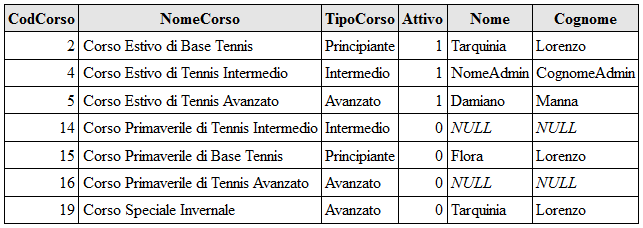
\includegraphics[width=\textwidth]{images/Query1.PNG}
\caption{Output Query 1}
\end{figure}
\newpage
\section{Query 2}

Estrae le informazioni riguardanti il corso 4.\\

\lstinputlisting[language=SQL]{sql/query2.sql}

\begin{figure}[H]
 \centering
  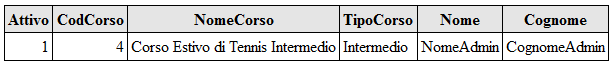
\includegraphics[width=\textwidth]{images/Query2.PNG}
\caption{Output Query 2}
\end{figure}

\newpage
\section{Query 3}

Estrae le prenotazioni fatte tra la data del 3 settembre ed il 4 settembre mostrando nome dell'utente associato o il nome dell'istruttore e del corso.\\

\lstinputlisting[language=SQL]{sql/query3.sql}

\begin{figure}[H]
 \centering
  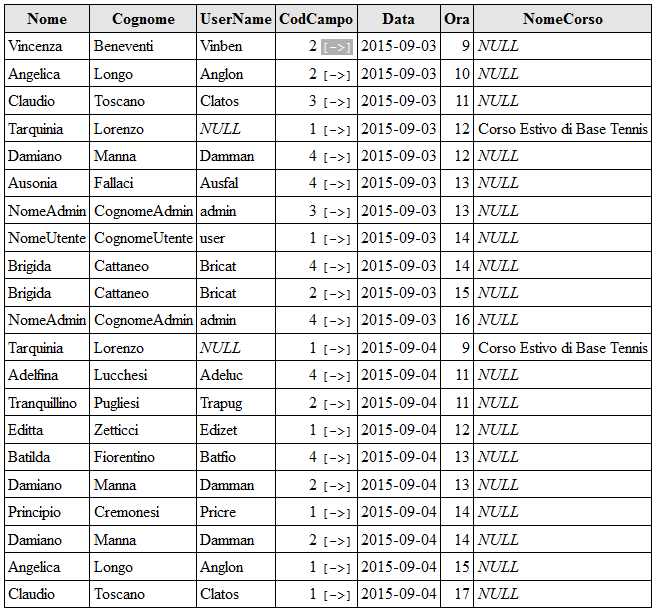
\includegraphics[width=\textwidth]{images/Query3.PNG}
\caption{Output Query 3}
\end{figure}

\newpage
\section{Query 4}
Restituisce, se c'e', una prenotazione per il campo 3 nella data 16-09-2015 alle ore 13.\\

\lstinputlisting[language=SQL]{sql/query4.sql}

\begin{figure}[H]
 \centering
  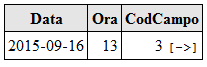
\includegraphics[width=0.5\textwidth, height= 5em]{images/Query4.PNG}
\caption{Output Query 4}
\end{figure}

\section{Query 5}
Estrae la lista delle lezioni del corso 2 e, se disponibili  anche le prenotazioni corrispondenti.\\

\lstinputlisting[language=SQL]{sql/query5.sql}

\begin{figure}[H]
 \centering
  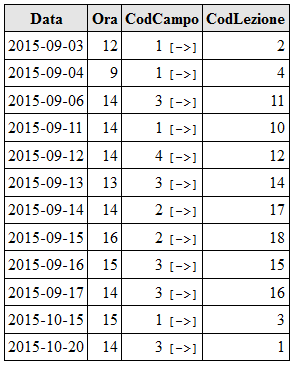
\includegraphics[width=0.5\textwidth]{images/Query5.PNG}
\caption{Output Query 5}
\end{figure}

\section{Query 6}

Estrae le informazioni di tutti i corsi attivi ai quali l'utente e' iscritto, con nome e cognome del rispettivo istruttore.\\

\lstinputlisting[language=SQL]{sql/query6.sql}

\begin{figure}[H]
 \centering
  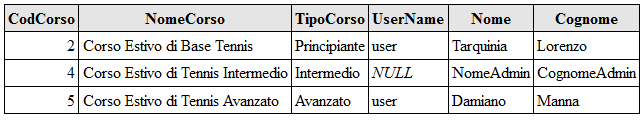
\includegraphics[width=\textwidth]{images/Query6.PNG}
\caption{Output Query 6}
\end{figure}

\section{Query 7}

Mostra le prenotazioni dell'utente che visualizza la pagina alla data indicata.\\

\lstinputlisting[language=SQL]{sql/query7.sql}

\begin{figure}[H]
 \centering
  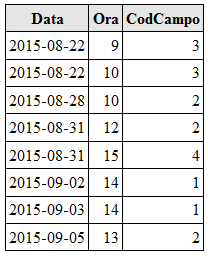
\includegraphics[width=0.5\textwidth]{images/Query7.PNG}
\caption{Output Query 7}
\end{figure}

\chapter{Trigger e Funzioni} 

\section{Trigger}

\subsection{InserimentoRetribuzione}
\lstinputlisting[language=SQL,firstline=98,lastline=110]{sql/DDL_Database.sql}

Il trigger controlla che la retribuzione di un istruttore non sia inferiore ad 800 euro, nel caso lo sia, imposta una retribuzione base di 800 euro.
Grazie a questo trigger viene espresso anche il vincolo semantico che la retribuzione di un istruttore non possa essere un valore negativo (minore o uguale a zero).

\subsection{AggiornaRetribuzione}
\lstinputlisting[language=SQL,firstline=112,lastline=124]{sql/DDL_Database.sql}

Trigger simile al precedente, utilizzato in caso di aggiornamento del campo retribuzione. Nel caso la retribuzione dell'istruttore venga impostata ad un valore sotto gli 800 euro, viene ripristinato il vecchio valore.

Sono stati necessari due trigger visto che MySQL non permette di definire trigger su condizioni multiple.

\subsection{CorsoAttivoIns}
\lstinputlisting[language=SQL,firstline=126,lastline=137]{sql/DDL_Database.sql}

Imposta un corso come non attivo se manca il codice fiscale dell'istruttore che lo tiene. Vale per l'inserimento di nuovi corsi.

\subsection{CorsoAttivoUpd}

\lstinputlisting[language=SQL,firstline=139,lastline=150]{sql/DDL_Database.sql}

Imposta un corso come non attivo se manca il codice fiscale dell'istruttore che lo tiene. Vale per l'aggiornamento dei corsi.

\newpage
\subsection{CorsoAttivoElim}

\lstinputlisting[language=SQL,firstline=152,lastline=166]{sql/DDL_Database.sql}

Come i trigger precedenti, si occupa di impostare il campo \textit{Attivo} di un corso a false (0) se viene eliminato l'istruttore che tiene quel corso.

\section{Funzioni}

\subsection{ControlloPrenotazione}

\lstinputlisting[language=SQL,firstline=173,lastline=192]{sql/DDL_Database.sql}

Controlla che un socio/istruttore non abbia altre prenotazioni personali nella stessa data e ora.
Controlla anche che nel caso l'utente sia un socio iscritto ad un corso oppure un istruttore che tiene un corso che la data e ora non coincidano con una prenotazione di una lezione gia' prenotata.

\subsection{ControlloPrenotazioneCorso}

\lstinputlisting[language=SQL,firstline=194,lastline=218]{sql/DDL_Database.sql}

Controlla che l'istruttore che tiene un corso non abbia gia' altre prenotazioni personali.

\newpage
\subsection{PossoIscrivermi}

\lstinputlisting[language=SQL,firstline=221,lastline=262]{sql/DDL_Database.sql}

Permette ad un socio di iscriversi solamente ad un corso compatibile al suo livello, tramite interfaccia web (mostrando o meno il pulsante di iscrizione).